\section{Registered results and post-result qualification}
\label{sec:results}

Both registrations' v0.4 development and confirmation ledgers record positive
classifications.  The
product walk passed all four development scenarios, all 16 development
witness groups, both confirmation scenarios, all eight confirmation witness
groups, and all four confirmation-state cross-witness groups.  The direct QCA
ledger classifier marked four of four development scenarios with 16 of 16
witness groups and two of two confirmation scenarios with eight of eight
witness groups as passing.  Each
committed development and confirmation ledger was accepted by the
algorithmically separate reconstruction as implemented.  The direct
$\pi$-sector predicate was later found to be empty in both primary and replay;
its measured values, associated pass flags, and one rough-potential control are withdrawn
(Sec.~\ref{sec:post-result-audit}).  The direct scenario counts are therefore
historical ledger classifications, not a claim that every intended registered
gate executed correctly.  No threshold or registered scientific input was
changed after confirmation opening.

\subsection{Certified convergence}

Figure~\ref{fig:convergence} plots every intact registered scenario-level
$d_N$ series; the withdrawn empirical $\pi$ reducer is a separate metric and
does not appear in this panel.  For the product walk, the largest certified
upper bounds across scenarios were $0.0300072572$, $0.0149954636$, and
$0.00749669028$ at $N=256,512,1024$.  The worst successive ratios were
$0.500088317$ and $0.500066986$, below the frozen $0.60$ gate.  The curves show
the registered first-order pattern without using a post-outcome slope fit as a
criterion.

For the direct QCA, the largest direct-only bounds were
$5.60191118\times10^{-4}$, $1.39960025\times10^{-4}$, and
$3.49845248\times10^{-5}$.  Their ratios lie between approximately $0.24984$
and $0.24997$, below the frozen $0.35$ gate and consistent with the analytic
second-order global discrepancy.  The largest potential-split bounds were
$2.75976665\times10^{-3}$, $1.37607978\times10^{-3}$, and
$6.87867299\times10^{-4}$, with ratios between approximately $0.49444$ and
$0.49987$, below $0.62$.  The active leading phase therefore produces the
separately anticipated first-order global family rather than being hidden
inside a direct-only convergence claim.

\begin{figure}[t]
  \centering
  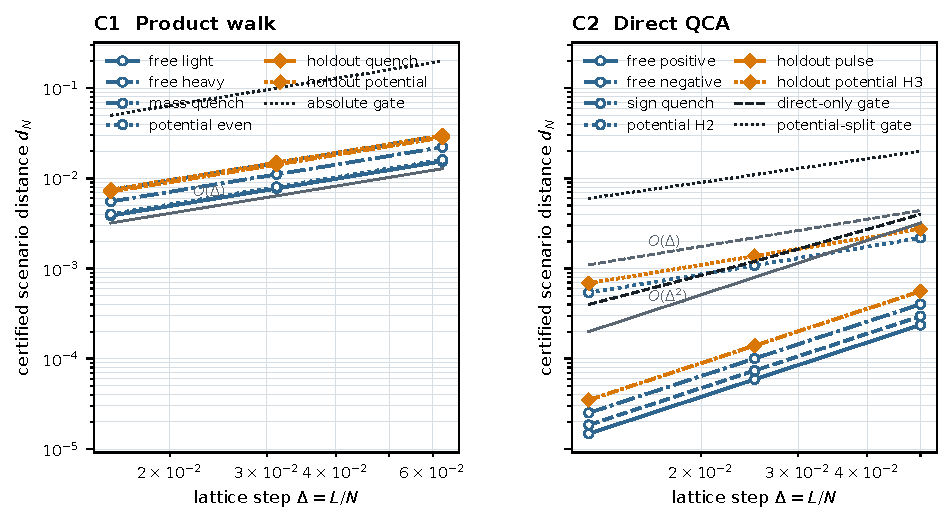
\includegraphics[width=\linewidth]{quantum_dirac_paper/figures/generated/fig03_certified_convergence.pdf}
  \caption{\textbf{Certified convergence of both frozen constructions
  (\registered).}  Each curve is the maximum over registered observation times
  of the serialized outward certified distance $d_N$ for one scenario,
  including its analytic tail and numerical budgets.
  Open markers denote development; filled diamonds denote single-use confirmation.
  The product panel retains its first-order gates; the direct panel retains
  distinct direct-only and potential-split gates.  Guide lines are analytic
  orders, not fits.  The updates have different frozen refinement and
  observation grids, and values are not normalized by their gates.}
  \label{fig:convergence}
\end{figure}

\subsection{Observable and structural witnesses}

The largest certified upper bound over development and confirmation for each
update is reported in Table~\ref{tab:witness-maxima}.  Product maxima remained
between about 11 and 249 times below their applicable gates; direct maxima
remained between about 72 and 876 times below their gates, depending on the
metric.  These margins are descriptive, not a cross-registration score: the
registrations have different steps, schedules, observation grids, and
threshold rationales.

\begin{table}[t]
  \centering
  \caption{Largest registered upper bounds for the six intact shared
  observable-witness families across both partitions.  Gates are absolute and
  were frozen separately.  The direct empirical $\pi$ value and pass flag are
  withdrawn and are not included in this table.}
  \label{tab:witness-maxima}
  \small
  % Generated table.
\begin{tabular}{@{}lrrrr@{}}
\toprule
Metric & Product max & Gate & Direct max & Gate \\
\midrule
Position TV & $0.00194047$ & $0.05$ & $9.8902\times 10^{-5}$ & $0.010$ \\
Momentum TV & $2.0061\times 10^{-4}$ & $0.05$ & $1.3971\times 10^{-4}$ & $0.010$ \\
Total-current error & $0.00844655$ & $0.10$ & $3.6737\times 10^{-5}$ & $0.020$ \\
Local-current $L_1$ & $0.00844655$ & $0.10$ & $1.9639\times 10^{-4}$ & $0.020$ \\
Infidelity & $4.5070\times 10^{-5}$ & $0.0025$ & $3.1546\times 10^{-7}$ & $0.0001$ \\
Zitterbewegung series $L_\infty$ & $0.00881467$ & $0.10$ & $2.2840\times 10^{-5}$ & $0.020$ \\
\bottomrule
\end{tabular}

\end{table}

For the product walk, the largest witness norm residual was
$3.39037\times10^{-13}$, the largest structural norm residual was
$6.22285\times10^{-13}$, and the largest parity residual was
$5.79543\times10^{-14}$, all within $10^{-12}$.  The largest fine
time-reversal-role residual was $0.0134492$ within its $0.10$ gate and passed
the first-order refinement requirement.  Exact causal support and both
massless cone boundaries passed.  The primary and independent state vectors
had serialized disagreement zero at the registered comparison precision.

For the direct QCA, the largest parity and unitarity residuals were
$9.63632\times10^{-74}$ and $1.22268\times10^{-67}$.  Potential-split
time-reversal-role residuals refined from $0.00550361$ to $0.00137599$ and
passed their $0.62$ ratio rule and $0.020$ fine gate.  All six scenarios passed
the exact implementation-integrity and causal-support gates.  The largest
analytic $\pi$-tail bound was $1.83341\times10^{-164}$, below $10^{-24}$.
The empirical $\pi$ values are not evidence because of
Eq.~\eqref{eq:pi-sector-correct}.  The largest state disagreement between
primary and independent implementations on the remaining numerical families
was $\DirectIndependentMax$, below $10^{-11}$.

\subsection{Declared resources and boundary controls}

At the finest product refinement, a free $T=2$ run uses 128 macrosteps, 384
elapsed elementary layers, and 393,216 gates.  A registered active-potential
run uses 448 layers and 458,752 gates.  At the finest direct refinement, a
free run uses 160 macrosteps, 320 layers, and 409,600 gates; the harmonic-$2$
and harmonic-$3$ potential schedules use 400 and 416 layers and 512,000 and
532,480 gates.  These totals faithfully charge each sealed protocol clock.
They are not an efficiency head-to-head because $N$, schedules, accuracy gates,
and gate-fusion conventions differ.  At equal $N$ and macrostep count, the
frozen decompositions assign free depth and work $3,3N$ to the product walk and
$2,2N$ to the direct QCA.  Section~\ref{sec:architectures} shows why these
nonminimal counts are not compilation-invariant and support no hardware or
minimal-resource advantage.

Six direct-QCA controls ran only after the confirmation primary.  Five remain
informative: the exact
opposite-mass $\pi$-partner residual was $2.49490\times10^{-111}$; a high-$q$
control had operator distance $0.00791313$; the $|\mu|=1$ endpoint had zero
maximum group velocity; a $T=12$ low-band control had distance
$0.000821366$; and the hard-core versus canonical fermionic
double-occupation phases had distance $2$.  The rough-potential zero is
withdrawn; the corrected audit-only diagnostic is $3.4860\times10^{-8}$.
These non-gating controls characterize the boundary.  They cannot repair a
failed primary and do not broaden the result.
